\documentclass[9pt]{beamer}
\usepackage{styles/mypreamble}
%~~~~~~~~~~~~~~~~~~~~~~~~~~~~~~~~~~~~~~~~~~~~~~~~~~~~~~~~~~~~~~~~~~~~~~~~~~~~~~
\title{Алгоритмы машинного обучения}
\subtitle{Лекция 11. Линейные методы классификации}
\author{Владимир Кукушкин}
\institute{СПбГЭУ - 2020}
\date{\today}
%~~~~~~~~~~~~~~~~~~~~~~~~~~~~~~~~~~~~~~~~~~~~~~~~~~~~~~~~~~~~~~~~~~~~~~~~~~~~~~

\begin{document}

\titlepage

\section{Линейная регрессия}

\begin{frame}{Задача классификации}
\begin{itemize}
    \item Будем решать задачу классификации по $K$ классам.
    \item $y_i \in \mathcal{G}$, $\mathcal{G} = \{1, 2, \ldots, K\}$.
    \item $\delta: \sf{X} \rightarrow \mathcal{G}$ -- решающее правило (дискриминантная функция). Обычно $\delta(x) = \underset{k=1,\ldots,K}{\mathrm{arg\;max}}\delta_k(x)$ -- считаем по данному наблюдению некоторый скор для каждого класса и выбираем класс с максимальным скором.
    \item Под линейным методом будем понимать такой алгоритм, дискриминантная функция которого линейна по фичам.
\end{itemize}
    
\end{frame}

\begin{frame}{Переход от модели линейной регресии}
    \begin{itemize}
        \item Обозначим через $Y$ матрицу индикаторов размером $N\times K$. В каждой строчке матрицы стоит 0 в колонке, соответствующей классу $y_i$.
        \item То есть $Y_k = \mathds{1}(y=k)$ -- бинарный вектор, показывающий, принадлежит ли $y_i$ классу $k$ или нет.
        \item Для каждого вектора $Y_k$ решим задачу линейной регрессии: $\hat Y_k = \hat\beta_{k0} +\hat\beta_{k}^Tx$, $k=1,\ldots,K$. Вместе это всё можно записать в виде:
        $$\hat Y = X(X^TX)^{-1}X^TY$$.
        \item Результат применения модели к наблюдению $x$: $\hat f(x) = (1, x^T)\hat B$ -- $K$-мерный вектор.
        \item Окончательный ответ: $\hat G(x) = \underset{k=1,\ldots,K}{\mathrm{arg\;max}}\hat f_k(x)$.
        \end{itemize}
\end{frame}

\begin{frame}{Почему не подходит линейная регрессия}
\includegraphicsheight{0.5}{img/lin_reg_classification.jpg}

\begin{itemize}
    \item Сама область значений регресии -- $\mathbb{R}$ в принципе не подходит к классам 0, 1.
    \item Сама линейная модель слишком жёсткая. Иногда классы невозможно разделить линейной моделью (masking problem).
\end{itemize}    
\end{frame}

\begin{frame}{Пример. Masking problem.}
\begin{tabular}{cc}
     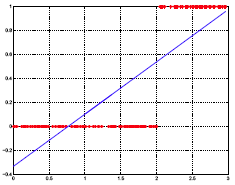
\includegraphics[height=0.45\textheight]{img/lin_reg_classification_masking_1.png}&
     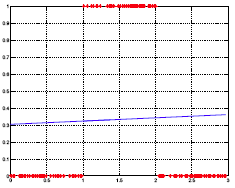
\includegraphics[height=0.45\textheight]{img/lin_reg_classification_masking_2.png}  \\
\end{tabular}
\begin{itemize}
    \item Левая картинка. Выбираем порог $x = 2$. Всё что левее -- класс 0, всё что правее -- класс 1.
    \item Правая картинка. Какой бы порог ни выбирали, мы не сможем отделить класс 1 -- он всегда будет сильно смешиваться с классом 0.
    \item Чем больше классов, тем сильнее проявление эффекта.
\end{itemize}
\end{frame}

\section{Линейный дискриминантный анализ}

\begin{frame}{Дискриминантный анализ}
\begin{itemize}
    \item Пусть $f_k$ -- плотности распределения фичей $X$ в классе $G = k$ и пусть $\pi_k$ -- априорные вероятности классов. Мы хотим посчитать $\text{Pr}(G|X)$ -- ожидаемые вероятности для каждого класса при условии наблюдать данные $X$.
    \item Эти вероятности можно посчитать через теорему Байеса:
    $$\text{Pr}(G=k \;|\; X = x) = \frac{\text{Pr}(X = x \;|\; G=k)\text{Pr}(G=k)}{\text{Pr}(X=x)} = \frac{f_k(x)\pi_k}{\sum_{l=1}^K f_l(x)\pi_l}.$$
    \item Будем предполагать, что фичи имеют нормальное распределение, то есть:
    $$f_k(x) = \frac{1}{(2\pi)^{1/2}|\Sigma_k|^{1/2}} e^{-\frac{1}{2}(x-\mu_k)^T\Sigma^{-1}(x-\mu_k)}.$$
\end{itemize}
\end{frame}

\begin{frame}{Дискриминант}
\begin{itemize}
    \item Если $\Sigma_k = \Sigma$ для всех $k$, то
    $$\delta_k(x) = x^T\Sigma^{-1}\mu_k -\frac{1}{2}\mu_k^T\Sigma^{-1}\mu_k + 
    \log\pi_k \text{--}$$
    линейный дискриминант (LDA -- Linear Discriminant Analysis).
    \item В общем случае дискриминант будет квадратичным (QDA -- Quadratic Discriminant Analysis):
    $$\delta_k(x) = -\frac{1}{2}\log |\Sigma_k| -\frac{1}{2}(x-\mu_k)^T\sigma_k^{-1}(x-\mu_k) + \log\pi_k.$$
    \item В качестве оценки параметров берём следующие выражения:
    \begin{itemize}
        \item $\hat \pi_k = N_k/N$, где $N_k$ -- количество наблюдений в классе $k$,
        \item $\hat \mu_k = \sum_{g_i = k}x_i / N_k$,
        \item $\hat \Sigma = \sum_{k=1}^K\sum_{g_i = k} (x-\hat\mu_k)(x-\hat\mu_k)^T/(N-K)$.
    \end{itemize}
\end{itemize}
\end{frame}

\begin{frame}{Решающее правило}
    \begin{itemize}
        \item В LDA удобно использовать отношение дискриминантов (a.k.a. log-odds):
        \begin{equation*}
        \begin{split}
            \log \frac{\text{Pr}(G=k \;|\; X = x)}{\text{Pr}(G=l \;|\; X = x)} = \log \frac{f_k(x)}{f_l(x)} + \log \frac{\pi_k}{\pi_l} = \\
            = \log \frac{\pi_k}{\pi_l} - \frac{1}{2}(\mu_k + \mu_l)^T\Sigma^{-1}(\mu_k-\mu_l) + x^T\Sigma^{-1}(\mu_k - \mu_l).
        \end{split}
        \end{equation*}
        \item Но можно использовать тот же $\underset{k=1,\ldots,K}{\mathrm{arg\;max}}\hat f_k(x)$. В частности, для двух классов \{1, 2\}, объект будет принадлежать классу 2, если
        $$x^T\Sigma^{-1}(\hat\mu_2-\hat\mu_1) > \frac{1}{2}\hat\mu_2^T\Sigma^{-1}\hat\mu_2 - \frac{1}{2}\hat\mu_1^T\Sigma^{-1}\hat\mu_1 + \log \frac{N_1}{N} - \log\frac{N_2}{N}.$$
        \item В QDA формула получается сложнее, поэтому проще вычислить $\underset{k=1,\ldots,K}{\mathrm{arg\;max}}\hat f_k(x)$ и всё.
    \end{itemize}
\end{frame}

\begin{frame}{Пример. LDA.}
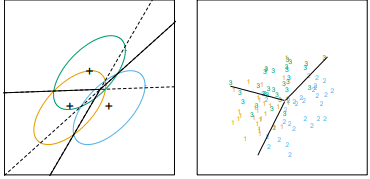
\includegraphics[width=\textwidth]{img/lda.png}
Сгенерировали три класса из двумерного нормального распределения. LDA даёт прямые границы между классами.
\end{frame}

\begin{frame}{Пример. QDA.}
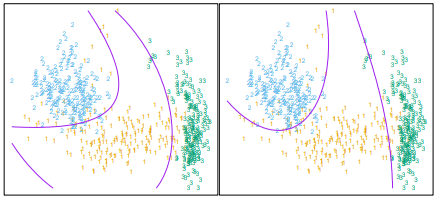
\includegraphics[width=\textwidth]{img/lda_qda.png}
\begin{itemize}
    \item Левая картинка -- границы LDA по фичам $X_1, X_2, X_1X_2, X_1^2, X_2^2$.
    \item Правая картинка -- границы QDA. 
\end{itemize}
\end{frame}

\section{Логистическая регрессия}

\begin{frame}{Идея}
\begin{itemize}
    \item Мы говорили о том, что нас не устраивала область значений модели линейной регрессии ($\mathbb{R}$). Хотелось бы, чтобы значения были из $[0, 1]$ и интерпретировались бы как вероятность принадлежности классу.
    \item Моделируем вероятности следующим образом:
    \begin{align*}
    \log \frac{\text{Pr}(G=1 \;|\; X = x)}{\text{Pr}(G=K \;|\; X = x)} &= \beta_{10} + \beta_1^Tx\\
    \log \frac{\text{Pr}(G=2 \;|\; X = x)}{\text{Pr}(G=K \;|\; X = x)} &= \beta_{20} + \beta_2^Tx\\
    \vdots& \\
    \log \frac{\text{Pr}(G=K-1 \;|\; X = x)}{\text{Pr}(G=K \;|\; X = x)} &= \beta_{(K-1)0} + \beta_{(K-1)}^Tx
    \end{align*}
\end{itemize}
\end{frame}

\begin{frame}{Решающее правило}
\begin{itemize}
    \item В предыдущей цепочке log-odds в знаменателях везде фиксирован класс $K$, но вместо него может использоваться любой, поскольку
    $$\text{Pr}(G=k\;|\; X=x) = \frac{\exp (\beta_{k0} + \beta_k^Tx)}{1+\sum_{l=1}^{K-1}\exp ( \beta_{l0} + \beta_l^Tx)}, k=1,\ldots, K-1$$
    $$\text{Pr}(G=K\;|\; X=x) = \frac{1}{1+\sum_{l=1}^{K-1}\exp(\beta_{l0} + \beta_l^Tx)}.$$
\end{itemize}
\end{frame}

\begin{frame}{Логистическая функция и сигмоида}
\begin{itemize}
    \item Функция $\log \frac{p}{1-p}$, где $p$ -- некоторая вероятность, называется логистической функцией (или логит-функцией). Сама дробь $\frac{p}{1-p}$ называется odds -- отсюда название log-odds.
    \item Функция преобразовывает $(0, 1)$ в $(-\inf, +\inf)$.
    \includegraphicsheight{0.5}{img/logit_function.png}
    \item Обратная функция -- $\frac{e^x}{1+e^x}$ называется сигмоидой.
\end{itemize}
\end{frame}

\subsection{Подгонка логистической регрессии}

\begin{frame}{Правдоподобие}
    \begin{itemize}
        \item Пусть $p_k(x_i, \beta) = \text{Pr}(G=k\;|\; X=x_i; \beta)$.
        \item В этом разделе будем рассматривать задачу подгонки модели для бинарной классификации. Классы будем кодировать через 0 и 1. Переобозначим $p(x_i, \beta) = p_1(x_i, \beta)$ и $p_2(x_i, \beta) = 1 - p(x_i, \beta)$.
        \item Логарифм правдоподобия записывается в виде
        \begin{equation}\label{logreg_loglike}
            \begin{split}
            l(\beta) = \sum_{i=1}^N \log p_{g_i} (x_i, \beta) = \sum_{i=1}^N \Big\{ y_i\log p_(x_i, \beta) + (1-y_i)\log(1-p(x_i, \beta))\Big\}=\\
            = \sum_{i=1}^N \Big\{ y_i\beta^T x_i - \log (1+e^{\beta^T x_i}) \Big\},
            \end{split}
        \end{equation}
        где $\beta = \{\beta_{10},\beta_1\}$ и к векторам $x_i$ добавляем фиктивную единицу первой компонентой, как делали в линейной регрессии.
    \end{itemize}
\end{frame}

\begin{frame}{Максимизация правдоподобия}
\begin{itemize}
    \item Будем максимизировать лог-правдоподобие \ref{logreg_loglike}.
    \item Производная правдоподобия
    $$\frac{\partial l(\beta)}{\partial\beta} = \sum_{i=1}^N x_i(y_i - p(x_i, \beta)) = 0$$
    \item Частные производные нелинейны по $\beta$, поэтому придётся использовать какой-нибудь приближённый алгоритм вычисления.
    \item Таким алгоритмом мог бы быть градиентный спуск, но поскольку мы можем посчитать вторые производные лог-правдоподобия \ref{logreg_loglike}, то лучше использовать метод Ньютона-Рафсона (улучшенный метод Ньютона, a.k.a. метод касательных).
    $$\frac{\partial^2 l(\beta)}{\partial \beta \partial \beta^T} = -\sum_{i-1}^N x_ix_i^T p(x_i, \beta)(1-p(x_i,\beta)),$$
    $$\beta^{\text{new}} = \beta^{\text{old}} - \left(\frac{\partial^2 l(\beta)}{\partial \beta \partial \beta^T}\right)^{-1} \frac{\partial l(\beta)}{\partial\beta},$$
    где все производные вычисляются для $\beta^{\text{old}}$.
\end{itemize}
\end{frame}

\begin{frame}{Регуляризация логистической регрессии}
\begin{itemize}
    \item Аналогично L1-регуляризации линейной регрессии, к правдоподобию \ref{logreg_loglike} можно добавлять штраф за большие значения коэффициентов:
    $$\max_{\beta_0,\beta} \Bigg\{ \sum_{i=1}^N \Big[ y_i\beta^T x_i - \log (1+e^{\beta^T x_i})\Big] -\lambda \sum_{j=1}^p |\beta_j| \Bigg\}.$$
    \item Оптимизируется также методом Ньютона-Рафсона (Koh, 2007).
\end{itemize}
    
\end{frame}

\begin{frame}[allowframebreaks]
    \frametitle{Литература}
    \bibliographystyle{unsrt}
    \nocite{esl}
    \bibliography{references.bib}
\end{frame}


\end{document}